%%%%%%%%%%%%%%%%%%%%%%%%%%%%%%%%%%%%%%%%%
% Structured General Purpose Assignment
% LaTeX Template
%
% This template has been downloaded from:
% http://www.latextemplates.com
%
% Original author:
% Ted Pavlic (http://www.tedpavlic.com)
%
% Note:
% The \lipsum[#] commands throughout this template generate dummy text
% to fill the template out. These commands should all be removed when 
% writing assignment content.
%
%%%%%%%%%%%%%%%%%%%%%%%%%%%%%%%%%%%%%%%%%

%----------------------------------------------------------------------------------------
%	PACKAGES AND OTHER DOCUMENT CONFIGURATIONS
%----------------------------------------------------------------------------------------

\documentclass{article}

\usepackage{fancyhdr} % Required for custom headers
\usepackage{lastpage} % Required to determine the last page for the footer
\usepackage{extramarks} % Required for headers and footers
\usepackage{graphicx} % Required to insert images
\usepackage{lipsum} % Used for inserting dummy 'Lorem ipsum' text into the template
\usepackage{amsmath,amsfonts,amsthm} % Math packages

% Margins
\topmargin=-0.45in
\evensidemargin=0in
\oddsidemargin=0in
\textwidth=6.5in
\textheight=9.0in
\headsep=0.25in 

\linespread{1.1} % Line spacing

% Set up the header and footer
\pagestyle{fancy}
\lhead{\hmwkAuthorName} % Top left header
\chead{\hmwkClass\ (\hmwkClassInstructor\ \hmwkClassTime): \hmwkTitle} % Top center header
\rhead{\firstxmark} % Top right header
\lfoot{\lastxmark} % Bottom left footer
\cfoot{} % Bottom center footer
\rfoot{Page\ \thepage\ of\ \pageref{LastPage}} % Bottom right footer
\renewcommand\headrulewidth{0.4pt} % Size of the header rule
\renewcommand\footrulewidth{0.4pt} % Size of the footer rule

\setlength\parindent{0pt} % Removes all indentation from paragraphs

%----------------------------------------------------------------------------------------
%	DOCUMENT STRUCTURE COMMANDS
%	Skip this unless you know what you're doing
%----------------------------------------------------------------------------------------

% Header and footer for when a page split occurs within a problem environment
\newcommand{\enterProblemHeader}[1]{
\nobreak\extramarks{#1}{#1 continued on next page\ldots}\nobreak
\nobreak\extramarks{#1 (continued)}{#1 continued on next page\ldots}\nobreak
}

% Header and footer for when a page split occurs between problem environments
\newcommand{\exitProblemHeader}[1]{
\nobreak\extramarks{#1 (continued)}{#1 continued on next page\ldots}\nobreak
\nobreak\extramarks{#1}{}\nobreak
}

\setcounter{secnumdepth}{0} % Removes default section numbers
\newcounter{homeworkProblemCounter} % Creates a counter to keep track of the number of problems

\newcommand{\homeworkProblemName}{}
\newenvironment{homeworkProblem}[1][Problem \arabic{homeworkProblemCounter}]{ % Makes a new environment called homeworkProblem which takes 1 argument (custom name) but the default is "Problem #"
\stepcounter{homeworkProblemCounter} % Increase counter for number of problems
\renewcommand{\homeworkProblemName}{#1} % Assign \homeworkProblemName the name of the problem
\section{\homeworkProblemName} % Make a section in the document with the custom problem count
\enterProblemHeader{\homeworkProblemName} % Header and footer within the environment
}{
\exitProblemHeader{\homeworkProblemName} % Header and footer after the environment
}

\newcommand{\problemAnswer}[1]{ % Defines the problem answer command with the content as the only argument
\noindent\framebox[\columnwidth][c]{\begin{minipage}{0.98\columnwidth}#1\end{minipage}} % Makes the box around the problem answer and puts the content inside
}

\newcommand{\homeworkSectionName}{}
\newenvironment{homeworkSection}[1]{ % New environment for sections within homework problems, takes 1 argument - the name of the section
\renewcommand{\homeworkSectionName}{#1} % Assign \homeworkSectionName to the name of the section from the environment argument
\subsection{\homeworkSectionName} % Make a subsection with the custom name of the subsection
\enterProblemHeader{\homeworkProblemName\ [\homeworkSectionName]} % Header and footer within the environment
}{
\enterProblemHeader{\homeworkProblemName} % Header and footer after the environment
}
   
%----------------------------------------------------------------------------------------
%	NAME AND CLASS SECTION
%----------------------------------------------------------------------------------------

\newcommand{\hmwkTitle}{Homework\ \#6} % Assignment title
\newcommand{\hmwkDueDate}{Wednesday,\ December\ 2,\ 2013} % Due date
\newcommand{\hmwkClass}{CS4642} % Course/class
\newcommand{\hmwkClassTime}{3:00pm} % Class/lecture time
\newcommand{\hmwkClassInstructor}{Hongyuan Zha} % Teacher/lecturer
\newcommand{\hmwkAuthorName}{Nathan Korzekwa} % Your name

%----------------------------------------------------------------------------------------
%	TITLE PAGE
%----------------------------------------------------------------------------------------

\title{
\vspace{2in}
\textmd{\textbf{\hmwkClass:\ \hmwkTitle}}\\
\normalsize\vspace{0.1in}\small{Due\ on\ \hmwkDueDate}\\
\vspace{0.1in}\large{\textit{\hmwkClassInstructor\ \hmwkClassTime}}
\vspace{3in}
}

\author{\textbf{\hmwkAuthorName}}
\date{} % Insert date here if you want it to appear below your name

%----------------------------------------------------------------------------------------

\begin{document}

\maketitle

%----------------------------------------------------------------------------------------
%	TABLE OF CONTENTS
%----------------------------------------------------------------------------------------

%\setcounter{tocdepth}{1} % Uncomment this line if you don't want subsections listed in the ToC

\newpage
\tableofcontents
\newpage

%----------------------------------------------------------------------------------------
%	PROBLEM 1
%----------------------------------------------------------------------------------------

% To have just one problem per page, simply put a \clearpage after each problem
``Your trivial words of sorrow, of love and guilt mean nothing to me, young lady. My wife understands. She is the one that I chose to live by my side. There are no more words that need to pass between us now. That's what it means to be the wife of the Fuhrer." -- Fuhrer-President King Bradley
\begin{homeworkProblem}[Problem 1]
	$$
		f(\vec{x}) = x_1^2 - 2x_1 + x_2^2 - x_3^2 + 4x_3
	$$
	
	$$
	\nabla f = \left[ \begin{array}{c}
	2x_1 - 2 \\
	2x_2\\
	-2x_3 + 4
	\end{array}
	\right]
	$$
	
	$$
		\nabla f(x^\star) = \left[ \begin{array}{c}
		3 \\
		-3 \\
		6
		\end{array}
		\right]
	$$
	
	The feasible directions $s$ point along the line defined by the constraint function, so 
	$$
	\vec{s} = \pm\left[\begin{array}{c}
		1\\
		3\\
		1
	\end{array}\right]
	$$
	
	Now let's check the first condition:
	$$
	\nabla f(x^\star)^T s = 3 - 9 + 6 = 0
	$$
	So, the first condition passes. Now, we calculate the Hessian to check the second:
	$$
	H_f = \left[\begin{array}{ccc}
	2 & 0 & 0 \\
	0 & 2 & 0 \\
	0 & 0 & -2
	\end{array}\right]
	$$
	
	$$
	s^TH_fs = 18
	$$
	so, this works out too. Note that we need not worry about the direction of $s$ in this case since a change in sign will cancel itself.
\end{homeworkProblem}
\clearpage
%----------------------------------------------------------------------------------------
%	PROBLEM 2
%----------------------------------------------------------------------------------------

\begin{homeworkProblem}[Problem 2] % Custom section title
%--------------------------------------------
\begin{homeworkSection}{(a)} % Section within problem
	Newton's iteration uses a second-order Talyor expansion of the form 
	$f(\vec{x} + \vec{s}) = f(\vec{x}) + \nabla f(\vec{x})\vec{s} + \frac{1}{2} \vec{s}^T H_f(\vec{x})\vec{s}$, which is minimized at each step by solving a linear system. However, the particular equation in this problem is quadratic itself, and thus can be modeled perfectly by a 2nd-order taylor expansion such as the one Newton's method uses. Therefore, it takes only one step for Newton's method to converge.
\end{homeworkSection}

\begin{homeworkSection}{(b)} % Section within problem
	If $x_0 - x^\star$ is an eigenvector of $A$, $x_0 - x^\star$ becomes the direction of steepest descent, and the problem convergences instantly.
\end{homeworkSection}
%--------------------------------------------
\end{homeworkProblem}
\clearpage

%----------------------------------------------------------------------------------------
%	PROBLEM 3
%----------------------------------------------------------------------------------------

\begin{homeworkProblem}[Problem 3] % Roman numerals
	\begin{homeworkSection}{(a)}
		To solve constrained problems such as this, one method is to construct a Lagrange function such that all critical points of this minimize the original function in the feasible space set by the constraining functions. In this problem, the Lagrange function is: 
		$$
			\mathcal{L}(x, y, \lambda) = x^2 + y^2 + \lambda y^2 - \lambda (x - 1)^3
		$$
		Our goal is to find where $\nabla \mathcal{L} = 0$. As a consequence of this, we must find a point where $-\nabla f = \lambda \nabla g$. However, if we look at the point $(1, 0)$, which happens to be a minimizer of $\mathcal{L}$, this property cannot hold since $\nabla g(1, 0) = 0$ and $\nabla f(1, 0) = [2, 0]^T$. This is because the constraint function $g$ is not smooth at that point. As a general rule, the Lagrange method will fail to find such points, possibly missing out on a local minimum. To solve problems with such constraint functions, we must resort to other methods.
		
	\end{homeworkSection}
	
	\begin{homeworkSection}{(b)}
		We transform the previous problem into a penalty problem. 
		\begin{align*}
			z(x,y) = x^2 + y^2 + \frac{1}{2}\rho[y^2-(x-1)^3]^2 \\
			\nabla z(x,y) = \left[\begin{array}{c}
					2x + \frac{1}{2}\rho[-6y^2(x-1)^2 + 6(x-1)^5] \\
					2y + \frac{1}{2}\rho[4y^3 - 4y(x-1)^3] \\
					\end{array}\right]\\
		\end{align*}
		
		Let's solve the second equation for $x$:
		\begin{align*}
			2\rho y(x-1)^3 = 2y + 2\rho y^3 \\
			(x - 1)^3 = \frac{2y + 2\rho y^3}{2\rho y}\\
			(x - 1)^3 = \frac{1}{\rho} + y^2\\
			(x - 1) = [\frac{1}{\rho} + y^2]^{1/3}\\
			x = [\frac{1}{\rho} + y^2]^{1/3} + 1\\
		\end{align*}
		
		So we find where the gradient of $z$ is zero, in terms of $x$ and $y$.
		First, we factor:
		$$
			2y + \frac{1}{2}\rho[4y^3 - 4y(x-1)^3] = y(2 + \frac{1}{2}\rho[4y^2 - 4(x-1)^3])
		$$
		and we know we can set $y = 0$.\\
		
		So we plug $y = 0$ into the equation we solved for $x$ earlier:
		$$
			x = \rho^{-\frac{1}{3}} + 1
		$$
		
		So, we obtain the critical point:
		$$
		\vec{v} = \left[\begin{array}{c}
				\rho^{-\frac{1}{3}} + 1\\
				0 \\
				\end{array}\right]
		$$
		
		... aaaannnddd
		$$
			\lim\limits_{\rho \rightarrow \infty} \vec{v} = \left[\begin{array}{c}
															1\\
															0 \\
															\end{array}\right]
		$$
		
		which is precisely the minimum that the Lagrange method failed to find earlier.
		
	\end{homeworkSection}
\end{homeworkProblem}
\clearpage
%----------------------------------------------------------------------------------------
%	PROBLEM 4
%----------------------------------------------------------------------------------------

\begin{homeworkProblem}[Problem 4] % Roman numerals
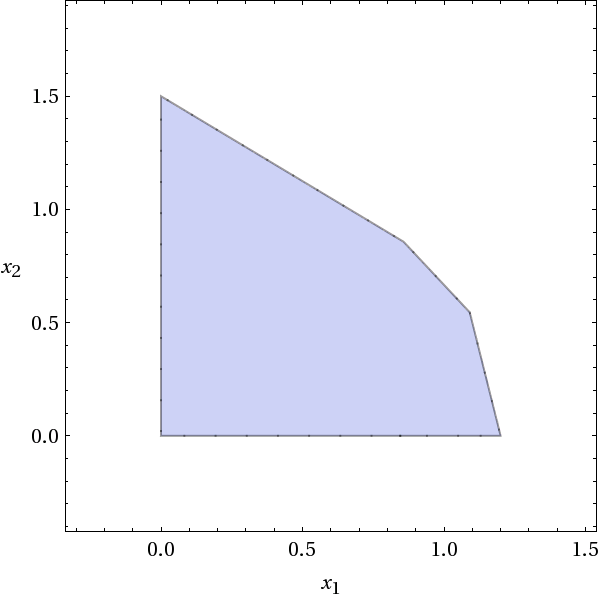
\includegraphics{q4plot}
\begin{homeworkSection}{(a)} % Section within problem
	The region has 5 vertices.
\end{homeworkSection}

\begin{homeworkSection}{(b)} % Section within problem
	The vertices are $x = (0, 1.5)^T$, $x = (6/5, 0)^T$, $x = (0, 0)^T$, $x = (6/7, 6/7)^T$, $x = (12/11, 6/11)^T$. The objective function at the previous points respectively: $-3$, $-18/5$, $0$, $-30/7$, $-48/11$. The minimum of these is $-48/11$, so $x = (12/11, 6/11)^T$ is the solution to this linear programming problem.
\end{homeworkSection}

\begin{homeworkSection}{(c)} % Section within problem
	Contours for the solutions at the vertices. The red line denotes the minimum of the objective function.
	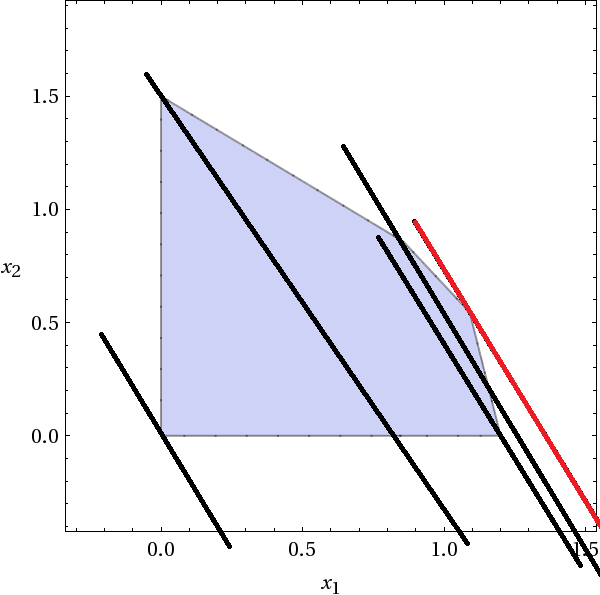
\includegraphics{q4plot2}
\end{homeworkSection}

\end{homeworkProblem}
\clearpage
%----------------------------------------------------------------------------------------

%----------------------------------------------------------------------------------------
%	PROBLEM 5
%----------------------------------------------------------------------------------------

\begin{homeworkProblem}[Problem 5] % Roman numerals
The code for this problem is included in the attached zip file as ``q5.m''.

\begin{homeworkSection}{(a)} % Section within problem
	This part of the problem is pretty self-explanatory. The method converged surprisingly quickly to 
	$$
	\vec{x} = \left[\begin{array}{c}
		14.3766 \\
		-1.5139 \\
	\end{array}\right]\\
	$$.	
\end{homeworkSection}

\begin{homeworkSection}{(b)} % Section within problem
	This part of the problem is a little less straight-forward than the previous one. Here, we are essentially transforming the problem into a mostly-linear problem that has the same minimizer $\vec{x}$. As a result, we are minimizing $log(x_1) + x_2t$. In this problem, I first solve the linear least squares problem:
	$$
	\left[\begin{array}{cc}
	 1 & 0.5\\
	 1 & 1\\
	 1 & 1.5\\
	 1 & 2\\
	 1 & 2.5\\
	 1 & 3\\
	 1 & 3.5\\
	 1 & 4\\
	\end{array}\right]x' \cong log(\vec{y})\\
	$$
	And since $x'_1$ represents $log(x_1)$, we can get $\vec{x} = [exp(x'_1), x'_2]^T$, to get the solution $\vec{x}$. Unfortunately, this transformation creates a problem. As can be seen from the included code, the two solutions are quite different. Since this is a least-squares problem, the solutions will seldomly be exact. As a consequence, the problem transformation creates a different residual functions for each problem. Since both of these residuals have different minima, the solutions to the two problems differ -- in this case, quite significantly.
\end{homeworkSection}
\end{homeworkProblem}
\clearpage

%----------------------------------------------------------------------------------------
%	PROBLEM 6
%----------------------------------------------------------------------------------------

\begin{homeworkProblem}[Problem 6] % Roman numerals

\begin{homeworkSection}{(a)}
	The function here is $f(x,y) = 2x^3-3x^2-6xy(x-y-1)$. So, to find the critical points, we try to find where $\nabla f = 0$. \\
	$$
	\nabla f = \left[\begin{array}{c}
		6x^2 - 6x -12xy +6y^2 + 6y \\
		-6x^2 + 12xy +6x \\
		\end{array}\right]\\
	$$
	
	So, we must find where both of these equations are equal to zero. We see right away that $-6x^2 + 12xy +6x = 6x(-x + 2y + 1)$, so we know that $x = 0$ in one or more critical points. Substituting $x = 0$ into the first equation, we find: $6y^2 + 6y = 0$, which can be factored into $6y(y+1) = 0$. So, for $x = 0$, $y = 0, -1$. Now we have two critical point found: $(0, 0)$ and $(0, -1)$. Now, notice if $y = 0$, then both equations are only left with $-6x^2 + 6x$, making $(1, 0)$ yet another critical point. Finally, through inspection, we can see that $(-1, -1)$ is a critical point.
\end{homeworkSection}

\begin{homeworkSection}{(b)}
	To analyze the critical points in this section, we first must calculate the Hessian matrix for $f$:
	$$
		H_f(x, y) = \left[\begin{array}{cc}
			12x - 6 - 12y & -12x + 12y + 6 \\
			-12x + 12y + 6 & 12x\\
			\end{array}\right]\\
	$$\\
	
	For critical point $(-1, -1)$:
	The Hessian at $(-1, -1)$ is 
	$$
		H_f(-1, -1) = 
			\left[\begin{array}{cc}
			-6 & 6 \\
			 6 & -12\\
			\end{array}\right]\\
	$$
	This matrix has the characteristic polynomial $\lambda^2 + 18\lambda + 36 = 0$, and by examining the quadratic equation, we see that both roots are negative. As a consequence, both eigenvalues are negative, meaning that this Hessian is negative-definite. Since this means that in all directions from this point the gradient becomes negative, this critical point is a local maximum. \\
	
	For critical point $(0, -1)$:
	The Hessian at $(0, -1)$ is 
	$$
		H_f(0, -1) = 
			\left[\begin{array}{cc}
			6 & -6 \\
		 -6 & 0\\
			\end{array}\right]\\
	$$
	This matrix has the characteristic polynomial $\lambda^2 + 6\lambda + 36 = 0$, and by examining the quadratic equation, we see that this equation has one positive and one negative root. Therefore, the eigenvalues are of opposite signs as well, so the matrix here is \textit{indefinite}, making this critical point a saddle point. \\
	
	For critical point $(1, 0)$:
	The Hessian at $(1, 0)$ is 
	$$
		H_f(1, 0) = 
			\left[\begin{array}{cc}
			 6 & -6 \\
			 -6 & 12\\
			\end{array}\right]\\
	$$
	This matrix is the additive inverse of the Hessian at $(-1, -1)$. As a consequence, both of it's eigenvalues are positive, making this matrix positive definite, meaning this critical point is a local minimum.
	
	For critical point $(0, 0)$:
		The Hessian at $(0, 0)$ is 
		$$
			H_f(0, 0) = 
				\left[\begin{array}{cc}
				-6 & 6 \\
			 6 & 0\\
				\end{array}\right]\\
		$$
		This matrix is the additive inverse of the Hessian at $(0, -1)$. However, that matrix was indefinite, since it had eigenvalues of opposite sign. Since negation preserves this property, this matrix is also indefinite.\\
\end{homeworkSection}

\begin{homeworkSection}{(c)}
	Observe the plot for the given function. Critical points are denoted by blue circles: \\
	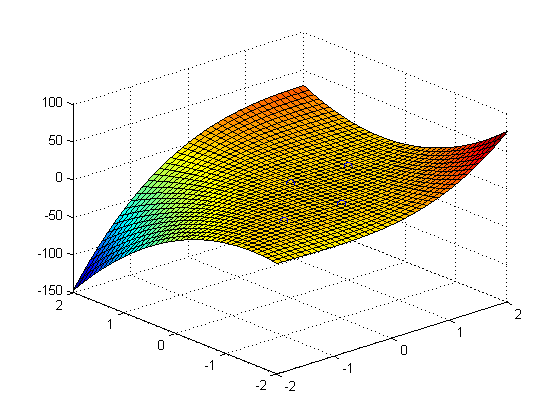
\includegraphics{q6plot} \\
\end{homeworkSection}

\begin{homeworkSection}{(d)}
	Using MATLAB's ``fminsearch'' I started with a large variety of starting vectors on $f$, with most of them converging, sensibly, to $[1, 0]^T$. However, a few diverged, with the function never reaching a critical point.
	
	The code for these trials is in a file named ``q6.m'' and is included in the zip file.
\end{homeworkSection}


\end{homeworkProblem}
\clearpage
%----------------------------------------------------------------------------------------
%	PROBLEM 7
%----------------------------------------------------------------------------------------

\begin{homeworkProblem}[Problem 7] % Roman numerals
	\begin{homeworkSection}{(a)}
		If $\vec{x}$ is a minimizer of a function $f$, then $f(\vec{x} + \epsilon\vec{v}) \geq f(\vec{x})$ for all $\vec{v}$ for a sufficiently small $\epsilon$ (equation(1)). \\
		
		Now if we assume that $f$ is convex and that $\vec{y}$ is also a local minimizer such that $f(\vec{y}) < f(\vec{x})$, then we know there exists some $\alpha$ s.t. $f(\alpha\vec{x} + (1 - \alpha)\vec{y}) > \alpha f(\vec{x}) + (1 - \alpha)f(\vec{y})$, because the line $\alpha f(\vec{x}) + (1 - \alpha)f(\vec{y})$ is bound by $\alpha f(\vec{x}) + (1 - \alpha)f(\vec{y}) \leq f(\vec{x})$, and equation (1) earlier guarantees a point $\vec{w}$ such that $f(\vec{w}) > f(\vec{x})$ from any line pointing out to another minimum. As a consequence, having another minimum contradicts the assumption that the function is convex. The two properties cannot both be present, thus proving that a convex function must have only one local minimum.
	\end{homeworkSection}
	
	\begin{homeworkSection}{(b)}
		For a function to be \textit{strictly} convex, then $f(\alpha\vec{x} + (1 - \alpha)\vec{y}) < \alpha f(\vec{x}) + (1 - \alpha)f(\vec{y})$ for all $\vec{x}, \vec{y} \ \epsilon S$ (where $S$ is a convex feasible set) and $0 < \alpha < 1$. For there to be a duplicate local minimum of an established minimum $\vec{x_1}$, there must exist another point $\vec{x_2}$ such that $f(\alpha\vec{x} + (1 - \alpha)\vec{y}) = \alpha f(\vec{x}) + (1 - \alpha)f(\vec{y})$ (equation (2)). This is because if all local neighbors of a minimum are greater, then any other value equal to $f(\vec{x_1})$ is a different local minimum. This is a consequence of equation (1). If any of the local neighbors are less than the local minimum, then there is a contradiction. Therefore, the requirement of equation (2) contradicts the definition of strictly convex, proving that strictly convex functions cannot have duplicate local minima.
	\end{homeworkSection}
\end{homeworkProblem}
\clearpage
\end{document}
